\documentclass{article}

% Language setting
% Replace `english' with e.g. `spanish' to change the document language
\usepackage[T2A]{fontenc}
\usepackage[utf8]{inputenc}

% Set page size and margins
% Replace `letterpaper' with `a4paper' for UK/EU standard size
\usepackage[letterpaper,top=2cm,bottom=2cm,left=3cm,right=3cm,marginparwidth=1.75cm]{geometry}

% Useful packages
\usepackage{amsmath}
\usepackage{graphicx}
\usepackage{float}
\usepackage[colorlinks=true, allcolors=blue]{hyperref}

\title{Лабораторная работа №4}
\author{Выполнили: Цалов В.С. Тахватулин М.В.}

\begin{document}
\maketitle
\begin{center}
      {\fontsize{14}{15}\selectfont
            Преподователь: Оранский С.И.
      }
\end{center}

% \title{Вариант 4}

\section{Задание}\label{sec:-no1}
\subsection{Текст задания}\label{subsec:-2}
Во всех вариантах требуется:

- построить модель линейной регрессии с указанными параметрами своими средствами (вместе со свободным коэффициентом),
то есть пользоваться готовыми линейными моделями нельзя (максимум - для сравнения своего результата с готовой
реализацией, плюс можно использовать NumPy для матричных вычислений или специальные функции, решающие оптимизационные
задачи);

- рассчитать оценки наименьших квадратов для параметров и остаточной дисперсии;
- вычислить коэффициент детерминации;
- построить доверительные интервалы для параметров модели и остаточной дисперсии;
- проверить гипотезы при уровне значимости \alph = 0,05 (формализовать основную и альтернативную гипотезу, рассчитать
статистику критерия, вычислить критические значения, указать p-value).


Зависимая переменная - цена на трансферном рынке, независимые - общий рейтинг, максимальный рейтинг на одной позиции,
возраст

Задачи про гипотезы:\newline
– Чем меньше возраст, тем больше цена.\newline
– Цена зависит от рейтинга.\newline
– Цена одновременно зависит от потенциального рейтинга и возраста.\newline

\subsection{Выполнение}\label{subsec:3}

В ходе выполнения задания мы построили модель линейной регрессии и нашли ее коэффициенты:

$Y = X * \beta + b$, где $\beta = (X^T * X)^{-1} * X^T * Y$

Далее нашли остаточную дисперсию (но она получилась слишком большой, т.к. зависимая переменная (цена) слишком большая):

$D = \frac{\sum^n_{i=1}(y_i - \dot{y_i} )^2}{N}$

И коэффициент детерминации:

$R^2 = \frac{\sum^n_{i=1}(y_i - \dot{y_i} )^2}{\sum^n_{i=1}(y_i - \bar{y_i} )^2}$

Затем нашли доверительные интервалы:

$\beta \pm t \cdot {std error}$

Проверили гипотезы:

$t = \frac{\beta}{std error}$ - t-статистика\newline
\newline
Из t-статистики мы посчитали p-значения, которые сравнили с уровнем значимости.
\newline\newline
– Чем меньше возраст, тем больше цена.\newline
Гипотеза 0: Чем меньше возраст, тем больше цена\newline
Гипотеза 1: Чем меньше возраст, тем меньше цена\newline
\newline
– Цена зависит от рейтинга.\newline
Гипотеза 0: Цена зависит от общего рейтинга\newline
Гипотеза 1: Цена не зависит от общего рейтинга\newline
\newline
– Цена одновременно зависит от потенциального рейтинга и возраста.\newline
Гипотеза 0: Цена одновременно зависит от максимального рейтинга и возраста\newline
Гипотеза 1: Цена одновременно не зависит от максимального рейтинга и возраста\newline


\subsection{Вывод программы}\label{subsec:-}

oстаточная дисперсия: 36752578051925.445

коэффициент детерминации (R^2): 0.6303883799511747\newline

доверительные интервалы:\newline
 [[-9.81950579e+02  7.94591426e+01]\newline
 [ 7.44766964e+05  7.78262804e+05]\newline
 [-3.50468306e+05 -3.10758256e+05]\newline
 [-4.02023606e+07 -3.83877071e+07]]\newline

гипотеза 0: Чем меньше возраст, тем больше цена\newline
гипотеза 1: Чем меньше возраст, тем меньше цена\newline
t-статистика: -84.88880289255964, p-значение: 2.0\newline
0 гипотеза принята\newline
\newline

гипотеза 0: цена зависит от общего рейтинга\newline
гипотеза 1: цена не зависит от общего рейтинга\newline
t-статистика: 89.12385662406068, p-значение: 2.0\newline
0 гипотеза принята\newline
\newline

гипотеза 0: цена одновременно зависит от максимального рейтинга и возраста\newline
гипотеза 1: цена одновременно не зависит от максимального рейтинга и возраста\newline
t-статистика возраста: -84.88880289255964, p-значение возраста: 2.0\newline
t-статистика максимального рейтинга: -32.638207789431995, p-значение максимального рейтинга: 2.0\newline
0 гипотеза принята\newline


\subsection{Программа}\label{subsec:2}
\begin{verbatim}

import numpy as np
import pandas as pd
import scipy.stats as stats
import matplotlib.pyplot as plt

data = pd.read_csv('fifa_players_stats.csv', delimiter=",", skiprows=1, names=[
    'Known As', 'Full Name', 'Overall', 'Potential', 'Value(in Euro)', 'Positions Played',
    'Best Position', 'Nationality', 'Image Link', 'Age', 'Height(in cm)', 'Weight(in kg)', 'TotalStats',
    'BaseStats', 'Club Name', 'Wage(in Euro)', 'Release Clause', 'Club Position', 'Contract Until',
    'Club Jersey Number', 'Joined On', 'On Loan', 'Preferred Foot', 'Weak Foot Rating', 'Skill Moves',
    'International Reputation', 'National Team Name', 'National Team Image Link', 'National Team Position',
    'National Team Jersey Number', 'Attacking Work Rate', 'Defensive Work Rate', 'Pace Total', 'Shooting Total',
    'Passing Total', 'Dribbling Total', 'Defending Total', 'Physicality Total', 'Crossing', 'Finishing',
    'Heading Accuracy', 'Short Passing', 'Volleys', 'Dribbling', 'Curve', 'Freekick Accuracy', 'LongPassing',
    'BallControl', 'Acceleration', 'Sprint Speed', 'Agility', 'Reactions', 'Balance', 'Shot Power', 'Jumping',
    'Stamina',
    'Strength', 'Long Shots', 'Aggression', 'Interceptions', 'Positioning', 'Vision', 'Penalties', 'Composure',
    'Marking', 'Standing Tackle', 'Sliding Tackle', 'Goalkeeper Diving', 'Goalkeeper Handling', 'GoalkeeperKicking',
    'Goalkeeper Positioning', 'Goalkeeper Reflexes', 'ST Rating', 'LW Rating', 'LF Rating', 'CF Rating', 'RF Rating',
    'RW Rating', 'CAM Rating', 'LM Rating', 'CM Rating', 'RM Rating', 'LWB Rating', 'CDM Rating', 'RWB Rating',
    'LB Rating', 'CB Rating', 'RB Rating', 'GK Rating'])

data['total_rating'] = data['ST Rating'] + data['LW Rating'] + data['LF Rating'] + data['CF Rating'] + \
                       data['RF Rating'] + data['RW Rating'] + data['CAM Rating'] + data['LM Rating'] + data[
                           'CM Rating'] + data['RM Rating'] + \
                       data['LWB Rating'] + data['CDM Rating'] + data['RWB Rating'] + data['LB Rating'] + data[
                           'CB Rating'] + \
                       data['RB Rating'] + data['GK Rating']

columns_to_max = ['ST Rating', 'LW Rating', 'LF Rating', 'CF Rating', 'RF Rating', 'RW Rating', 'CAM Rating',
                  'LM Rating', 'CM Rating', 'RM Rating', 'LWB Rating', 'CDM Rating', 'RWB Rating', 'LB Rating',
                  'CB Rating', 'RB Rating', 'GK Rating']
data['max_rating'] = data[columns_to_max].max(axis=1)

# y = x beta + b
X = data[['total_rating', 'max_rating', 'Age']].values
y = data['Value(in Euro)'].values

n, k = X.shape

X = np.column_stack([X, np.ones(n)])

# коэффициенты
beta = np.linalg.inv(X.T @ X) @ X.T @ y

# остаточная дисперсия
y_pred = X @ beta.T
N = n - k
dispersia = ((y - y_pred) ** 2).sum() / N
print("oстаточная дисперсия:", dispersia)


# коэффициент детерминации
y_srednee = y.mean()
total_sum = ((y - y_srednee) ** 2).sum()
total_sum_ostatki = ((y_pred - y_srednee) ** 2).sum()
r_square = 1 - (total_sum_ostatki / total_sum)
print("коэффициент детерминации (R^2):", r_square)


# доверительные интервалы
alpha = 0.05
t_value = stats.t.ppf(1 - alpha / 2, N)
st_er = np.sqrt(dispersia * np.diag(np.linalg.inv(X.T @ X)))
intervals = np.array([beta - t_value * st_er, beta + t_value * st_er]).T
print("доверительные интервалы:\n", intervals)


t_values = beta / st_er
p_values = stats.t.cdf(np.abs(t_values), N) * 2


# Гипотеза: Чем меньше возраст, тем больше цена
print(f"гипотеза 0: Чем меньше возраст, тем больше цена")
print(f"гипотеза 1: Чем меньше возраст, тем меньше цена")
print(f"t-статистика: {t_values[3]}, p-значение: {p_values[3]}")
if p_values[3] > alpha:
    print('0 гипотеза принята\n')
else:
    print('1 гипотеза принята\n')

# Гипотеза: Цена зависит от рейтинга
print(f"гипотеза 0: цена зависит от общего рейтинга")
print(f"гипотеза 1: цена не зависит от общего рейтинга")
print(f"t-статистика: {t_values[1]}, p-значение: {p_values[1]}")
if p_values[1] > alpha:
    print('0 гипотеза принята\n')
else:
    print('1 гипотеза принята\n')

# Гипотеза: Цена одновременно зависит от максимального рейтинга и возраста
print(f"гипотеза 0: цена одновременно зависит от максимального рейтинга и возраста")
print(f"гипотеза 1: цена одновременно не зависит от максимального рейтинга и возраста")
print(f"t-статистика возраста: {t_values[3]}, p-значение возраста: {p_values[3]}")
print(f"t-статистика максимального рейтинга: {t_values[2]}, p-значение максимального рейтинга: {p_values[2]}")
if p_values[3] > alpha and p_values[2] > alpha:
    print('0 гипотеза принята\n')
else:
    print('1 гипотеза принята\n')


plt.plot(data['total_rating'], data['Value(in Euro)'], 'o', color='red')
plt.xlabel('Общий рейтинг')
plt.ylabel('Цена')
plt.title('Цена от общего рейтинга')
plt.show()

plt.plot(data['max_rating'], data['Value(in Euro)'], 'o', color='green')
plt.xlabel('Максимальный рейтинг')
plt.ylabel('Цена')
plt.title('Цена от макс рейтинга')
plt.show()

plt.plot(data['Age'], data['Value(in Euro)'], 'o', color='orange')
plt.xlabel('Возраст')
plt.ylabel('Цена')
plt.title('Цена от возраста')
plt.show()

\end{verbatim}

\begin{figure}[H]
      \centering
      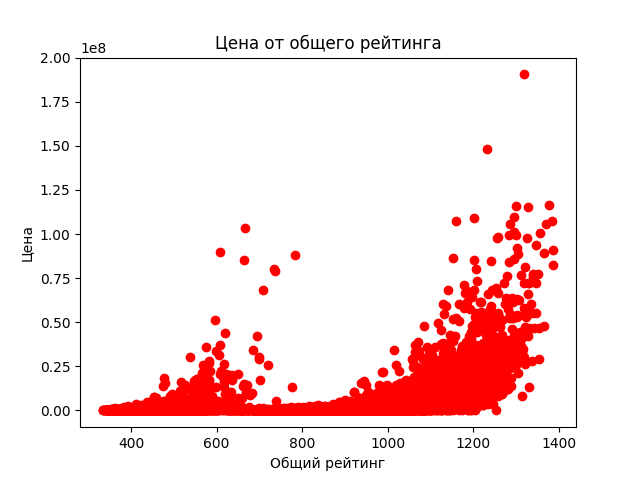
\includegraphics[width=0.7\linewidth]{total_rating}\label{fig:figure1}
\end{figure}

\begin{figure}[H]
      \centering
      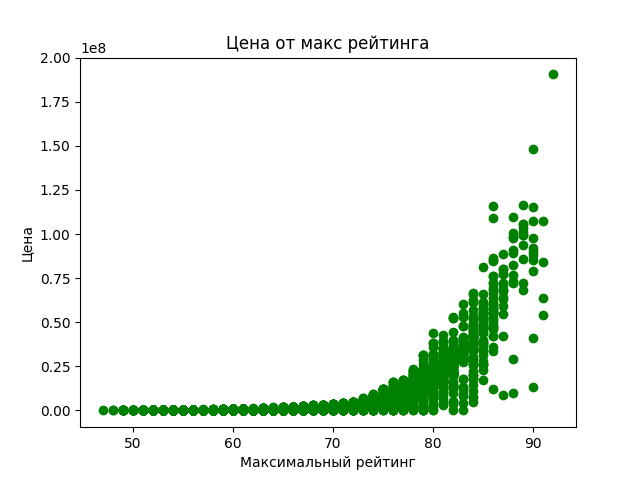
\includegraphics[width=0.7\linewidth]{max_rating}\label{fig:figure2}
\end{figure}

\begin{figure}[H]
      \centering
      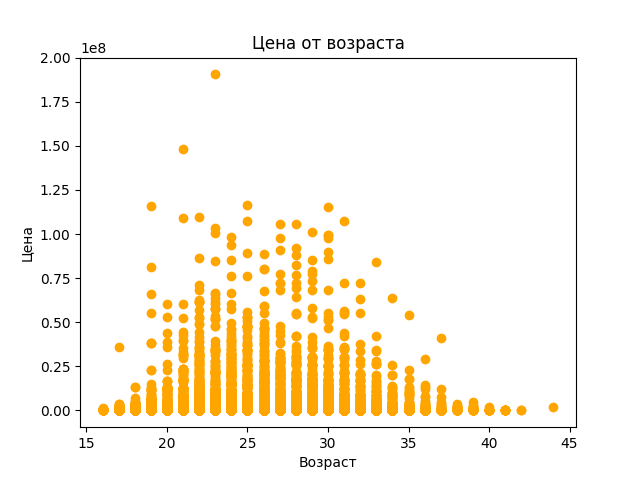
\includegraphics[width=0.7\linewidth]{age}\label{fig:figure3}
\end{figure}

\subsection{Описание результатов}\label{subsec:-3}
Все 0 гипотезы были приняты, так как значения p-значений больше уровня значимости, что означает линейную связь
зависимой переменной (цены футболиста) с независимыми переменными (общий рейтинг, максимальный рейтинг из всех
позиций, возраст)

\subsection{Вывод}\label{subsec:}

В процессе выполнения лабораторной работы, мы научились строить модель линейной регрессии по набору заданных параметров,
благодаря которым можно выявлять линейную связь между зависимыми и независимыми переменными.

\end{document}